% !TeX root = ./mfog-ieee.tex
% \documentclass{article}
% \documentclass[conference]{lib/IEEEtran}
\documentclass[conference]{IEEEtran}
\usepackage{babel}
\usepackage[utf8]{inputenc}
\IEEEoverridecommandlockouts
% The preceding line is only needed to identify funding in the first footnote. If that is unneeded, please comment it out.
\usepackage{xspace}
% \usepackage{cite}
\usepackage{amsmath,amssymb,amsfonts}
\usepackage{algorithmic}
\usepackage{graphicx}
\usepackage{textcomp}
\usepackage{xcolor}
% \def\BibTeX{{\rm B\kern-.05em{\sc i\kern-.025em b}\kern-.08em
%     T\kern-.1667em\lower.7ex\hbox{E}\kern-.125emX}}
\begin{document}

\title{IoT Intrusion Detection with Distributed Novelty Detection:
Design, Implementation and Evaluation [DRAFT]\thanks{CNPq}}

\author{
  \IEEEauthorblockN{Luís Puhl, Guilherme Weigert Cassales, Hermes Senger, Helio Crestana Guardia}
  \IEEEauthorblockA{Universidade Federal de São Carlos, Brasil \\
    Email: \{luispuhl, gwcassales\}@gmail.com, \{hermes@, helio@dc.\}ufscar.br
  }
  % \IEEEauthorblockN{Hermes Senger}\IEEEauthorblockA{\textit{Universidade Federal de São Carlos}, Brasil \\hermes@ufscar.br}\and
    % \IEEEauthorblockN{Guilherme Weigert Cassales}\IEEEauthorblockA{\textit{Universidade Federal de São Carlos}, Brasil \\gwcassales@gmail.com}
    % \and
    % \IEEEauthorblockN{4\textsuperscript{th} Given Name Surname}
    % \IEEEauthorblockA{\textit{dept. name of organization (of Aff.)} \\
    % \textit{name of organization (of Aff.)}\\
    % City, Country \\
    % email address or ORCID}
}

\maketitle

\begin{abstract}
  The implementation of the Internet of Things (IoT) is sharply increasing the small
  devices count and variety on edge networks and, following this increase the
  attack opportunities for hostile agents also increases, requiring more from
  the network administrator role and the need for tools to detect and react to those
  threats.
  % 
  One such tool are the Network Intrusion Detection Systems (NIDS) where the network
  traffic is captured and analysed raising alarms when a known attack pattern or
  new pattern is detected.
  For a network security tool to operate in the context of edge and
  IoT it has to comply with processing time, storage space and energy
  requirements alongside traditional requirements for stream and network
  analysis like accuracy and scalability.
  % 
  This work addresses the construction details and evaluation of an prototype
  distributed IDS using MINAS Novelty Detection algorithm
  following up the previously defined IDSA-IoT architecture.
  We discuss the algorithm steps, how it can be deployed in a distributed environment,
  the impacts on the accuracy of MINAS and evaluate the performance and scalability
  using a cluster of constrained devices commonly found in IoT scenarios.
  % 
  We found an increase of \textit{A 0.0} processed network flow descriptors per core
  added to the cluster. Also \textit{B 0.0\%} and \textit{C 0.0\%} change in
  \textit{F1Score} in the tested datasets when stream was unlimited in speed and
  limited to \textit{0.0 z MB/s} respectively.
\end{abstract}

\begin{IEEEkeywords}
% Detecção de Novidades, Detecção de Intrusão, Fluxos de Dados, Computação Distribuı́da, Computação em Névoa, Internet das Coisas.
novelty detection, intrusion detection, data streams, distributed system, edge computing, internet of things
\end{IEEEkeywords}

\section{Introduction}

% skel
  % The implementation of the Internet of Things (IoT) is sharply increasing the small
  % devices count and variety on edge networks and, following this increase the
  % attack opportunities for hostile agents also increases, requiring more from
  % the network administrator role and the need for tools to detect and react to those
  % threats.
  % % 
  % One such tool are the Intrusion Detection Systems (IDS) where the network
  % traffic is captured and analysed raising alarms when a known attack pattern or
  % new pattern is detected.
  % To build an IDS one option for base algorithm are
  % the Data Stream Novelty Detection being MINAS one of those.
  % % 
  % Furthermore, for a network security tool to operate in the context of edge and
  % IoT it has to comply with processing time, storage space and energy
  % requirements alongside traditional requirements for stream and network
  % analysis like accuracy and scalability.
  % % 
  % This work addresses the construction details and evaluation of an prototype
  % distributed IDS using MINAS Novelty Detection algorithm
  % following up the previously defined IDSA-IoT architecture.
  % We discuss the algorithm steps, how it can be deployed in a distributed environment,
  % the impacts on the accuracy of MINAS and evaluate the performance and scalability
  % using a cluster of constrained devices commonly found in IoT scenarios.
  % % 
  % We found an increase of \textit{A 0.0} processed network flow descriptors per core
  % added to the cluster. Also \textit{B 0.0\%} and \textit{C 0.0\%} change in
  % \textit{F1Score} in the tested datasets when stream was unlimited in speed and
  % limited to \textit{0.0 z MB/s} respectively.

\newcommand{\refminas}{\textit{Ref}\xspace}
\newcommand{\mfog}{\textit{MFOG}\xspace}
\newcommand{\iot}{IoT\xspace}

The advent of Internet of Things (\iot) is growing the count and diversity of
devices on edge networks, this growth increases network traffic patterns and
extends opportunities for cyber attacks presenting new challenges for network
administrators.
To address those challenges new Network Intrusion Detection Systems (NIDS) and
architectures can be explored, especially in Fog Computing and Data Stream (DS)
areas.

% Data Stream (DS)

% - Desafio, resposta, justificativa.
% - Artigo para setembro ou outubro.
% - Revisão dos valores da avaliação.

% ### Desafios, Respostas e Justificativas

% Desafios de arquitetura e validação:

% - Construção de um protótipo da arquitetura IDSA-IoT:
%   - Kafka (Python): Distribuição e balanceamento pelo cluster kafka, hipótese refutada.
%   - Flink (Java ou Scala): Execução do cluster nos dispositivos de névoa, hipótese refutada.
%   - MPI (C e Python): Execução do cluster nos dispositivos de névoa, hipótese aceita.
% - Reimplementação do algoritmo MINAS com fidelidade:
%   - Duas versões: a descrita e a implementação de referência (em Java).
%   - Resolução: utilizar a descrição, não *seguir* a imp. referência, apenas como ponto de comparação. Exemplos:
%     - Definição de raio `r = f * σ` (fator vezes desvio padrão) para `r = max(distance)` (distância máxima);
%     - Tamanho do buffer de desconhecidos e frequência de execução do passo de detecção de novidade;

Expected results:
A system that embraces and explores the inherent distribution of fog computing
in a IoT scenario opposing regular systems where data streams are collected and
centralized before processing;
Impact assessment of the impact of distributed, regional flow characteristics,
local vs global vs distributed forgetting mechanism and other polices.

IDS characteristics and description of physical scenario.

MINAS characteristics.

Distribution and IDSA-IoT architecture.

This paper is structured as follows:
Section \ref{sec:related} presents previous works that addresses related
problems and how they influenced our solution.
Section \ref{sec:implementation} address our proposal, the work done, issues
found during implementation and discusses parameters and configurations options
and how we arrived at our choices.
Section \ref{sec:experiments} shows experiments layouts and results, we
compare serial and distributed implementation's metrics for validation,
we also evaluate communication delay effects on classification metrics and
conclude with the speedup per core and overall maximum stream speed.
Section \ref{sec:conclusion} summarizes the research results and presents our
final conclusions and future works.


% ----------------------------------------------------------------------------------------------------------------------
\section{Related Work}\label{sec:related}

Recent works explored those areas, to name a few: BigFlow \cite{Viegas2019}
employing Apache Kafka and Apache Flink for distributed stream processing
evaluating with package stream dataset,
CATRACA \cite{Lopez2018,AndreoniLopez2019a} uses 
Apache Kafka and Apache Spark for stream processing and 

% ----------------------------------------------------------------------------------------------------------------------
\section{Implementation}\label{sec:implementation}

The original MINAS algorithm has a companion implementation (\refminas)
written in Java using MOA library base algorithms such as K-means and CluStream.
\refminas employs Java's double, a $64 bits$ number whose precision is not
absolutely necessary and, as it is often necessary to shuffle between nodes via
network and a small economy could be made with only a float number with $32 bits$.
Another difference between \refminas and \mfog is cluster radius calculation
from the distances of elements forming the cluster and the cluster's center,
where the former uses the maximum distance, the latter uses the standard deviation
of all distances as described in \cite{Faria2016minas}.

\begin{figure}[htbp]
\centerline{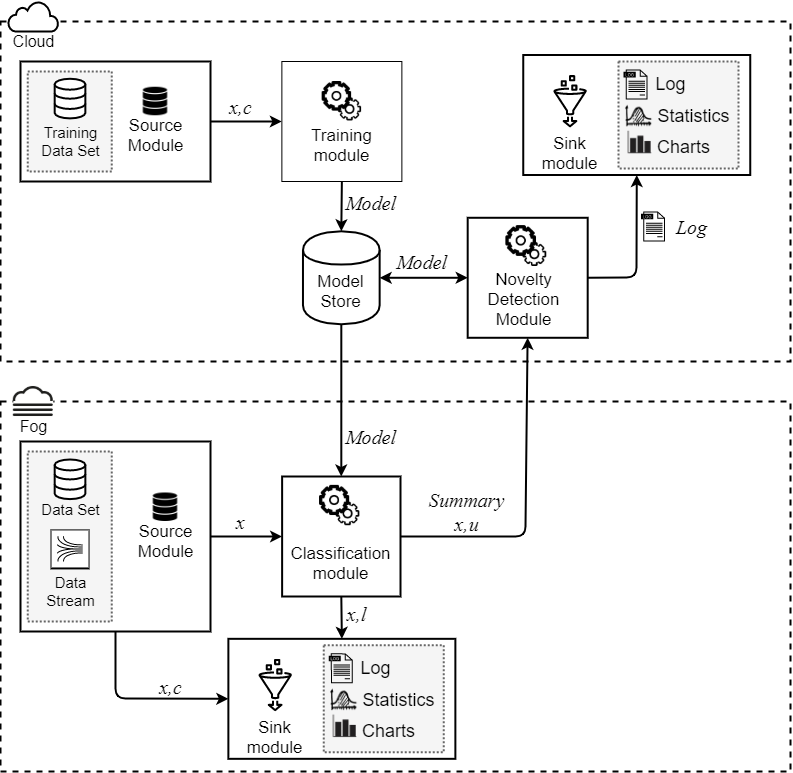
\includegraphics[width=0.45\textwidth]{figures/mfog-arch-v2_en.png}}
\caption{\mfog architecture overview.}
\label{fig:mfog-architecture}
\end{figure}

% Desafios de implementação:
% <!--
% - Definição de raio: desvio padrão das distâncias versus distancia máxima;
% - Atualização do micro-cluster limita-se à atualização do atributo \texttt{T};
% - Remoção de exemplos na implementação de referência é feita somente para o algoritmo \textit{CluStream};
% - Inclusão de borda: algoritmo inclui ($<=$), referência não inclui ($<$);
% - Seguiu-se as mesmas divergências anteriores para comparação dos resultados com a implementação referência;
% - Inclusão da borda;
% - Comportamento do mecânismo de \textit{sleep-model} não está definido, portanto não está ativo;
% - Processo de clusterização é limitado ao algoritmo \textit{K-Means}. Algoritmo \textit{CluStream} não está implementado;
% - -->
% - `Double vs Float`:
%   - Na implementação de referência, java double é utilizado;
%   - Na nova implementação duas versões foram testadas e a diferença de precisão entre as duas é de `5 E-8`;
%   - **Solução:** Use `float32` e economize os bits já que haverá comunicação entre nós e módulos;
% - Formato do fluxo de saída:
%   - Implementação de referência utiliza a tripla `(id, classe, etiqueta)`;
%   - Primeira implementação em C utiliza `(id, clusterLabel, clusterId, clusterRadius, label, distance, secondDistance)`;
%   - Segunda implementação utiliza dupla `(id, label)`;
%   - Na etapa de avaliação, independente de versão, o fluxo original é lido;
%   - **Solução:** O formato mínimo é `(id, label)`;

The stream format for input and output also of note.
Input information needed is the value of the item, this value is a number
sequence of length $d$ (referenced as dimension).
In addition to the value for evaluation and training purposes the class
identifier as single character, optimality an unique item identifier
(\textit{uid}) can be provided.
For output information and format the decision isn't so clear as we can't
predict future system integrations needs like only novelty alarms or every
item's original value with assigned label so, we have a compromise and put only
enough information for the Evaluation Module (where the full information
from the testing file or stream can de accessed) meaning the format can be
defined as a tuple containing \textit{uid} and assigned label.

% - Reprocessamento dos exemplos utilizados para atualização do modelo:
%   - Muda o comportamento do operador de fluxo de `Map` para `Flatmap`, ou seja,
%     requer outro fluxo de saída para a transmissão de padrões novidade (alarmes);
%   - Para reclassificação a definição de raio é modificada de `r = f * σ` (fator
%     multiplicando desvio padrão) para `r = max(distance)` (distância máxima);
%   - Passível da crítica de *overfitting*. Isto é, este processo pode
%     inflar a métrica de precisão;
%   - **Solução:** *em aberto*;

Another implementation decision related to the output stream is whether or not
to reprocess, and add to the output stream, examples in the unknown buffer after
the novelty detection procedure, meaning one item can be classified once as
unknown and again with a label.
Our tests using this technique had increased true positives when compared to
not using it.
However this changes the stream operator behavior from a \textit{Map} to a
\textit{FlatMap} having duplicate entries on the output stream as previously
mentioned.
Regardless of choice the classification of the unknown buffer after a model
update, using the full model or just the added set of clusters, is done to
remove the examples ``consumed'' in the creation of a new cluster in the internals
of the clustering algorithm.
% This removal can be made less complex if using only new clusters 

% Próximos desafios:
% - Distribuição e paralelização para minimização de latência entre novo item no fluxo e sua classificação:
%   - Tempo de passagem da instância pelo classificador;
%   - Volume máximo do sistema;
%   - Diferenças de precisão de acordo com a carga;

Polices

- Detecção de novidades e manutenção de modelo em ambiente distribuído:

  - Mecanismo de ND local (síncrono) vs nuvem quanto à atraso de definição de modelo
    (nesse ponto é onde a hipótese prevê maior diferença, grande ponto de interesse);

  - Mecanismo de esquecimento local vs global (modelo único ou por nó);

  - Atraso na reclassificação dos desconhecidos;


The Evaluation Module was also build following reference techniques like
multi-class confusion matrix with label-class association
\cite{Faria2016minas}
to extract classification quality metrics.

% ----------------------------------------------------------------------------------------------------------------------
\section{Experimental Setup and Results}\label{sec:experiments}

The experimental setup is composed of 2 environments and 3 datasets.
Kyoto December 2015.

\begin{quote}
  For the experiments, we used the Kyoto 2006+ dataset
  which contains data collected from 2006 to December 2015.
  We selected examples from one month, December, 2015. Only the examples of known
  attack types and known IDS alert code with a minimum of 10,000 occurrences (for
  significance) were considered. The offline training was performed with 72,000
  examples (i.e., 10\% of the dataset) using the holdout technique.
  \cite{Cassales2019a}
\end{quote}


% Minas with
  % filenameOffline = datasets/training.csv
  % filenameOnline = datasets/test.csv

  % outputDirectory = out/minas-og//2020-08-25T12-18-16.272
  % algClusteringOff = kmeans
  % algClusteringOnl = kmeans

  % threshold = 2.0
  % flagEvaluationType = 1
  % thresholdForgettingPast = 10000
  % numMicro = 100
  % flagMicroClusters = true

  % minExCluster = 20
  % validationCriterion = dec
  % isValidationCriterionDec = true

  % isGUIEnabled = false

  % Final Confusion Matrix: 
  % ,C N,N 1,N 2,N 3,N 4,N 5,N 6,N 7,N 8,N 9,N 10,N 11,N 12,N 13,N 14,Unk
  % C N,181391,0,13,0,43,0,0,314,97,826,13887,142,5793,35,10,3727
  % C A,437837,123,35,6,483,52,164,2,939,2133,3752,349,1121,0,39,144
  % ***
  % Impressao em forma de porcentagem: 
  % ,C N,N 1,N 2,N 3,N 4,N 5,N 6,N 7,N 8,N 9,N 10,N 11,N 12,N 13,N 14,Unk
  % C N,0.8793521364372352,0.0,6.30217473506627E-5,0.0,2.0845654892911506E-4,0.0,0.0,0.0015222175898544682,4.702391917703294E-4,0.004004304870126723,0.06732176965066561,6.883913941380079E-4,0.028083460184799156,1.6967393517486112E-4,4.847826719281746E-5,0.01806785018276307
  % C A,0.9791090368733774,2.7505763911096006E-4,7.826843389336261E-5,1.3417445810290734E-5,0.001080104387728404,1.1628453035585303E-4,3.667435188146134E-4,4.472481936763578E-6,0.0020998302693104997,0.004769901985558355,0.008390376113368472,7.804480979652443E-4,0.0025068261255559855,0.0,8.721339776688977E-5,3.220186994469776E-4
  % ***
  % FNew,MNew,Err
  % 12.064786,97.910904,70.8117
  % ***
  % Offline time 99.651
  % earlyReturn i=27
  % Online time 52.964
  % Results time 2.335
  % execution time 154.951

%    , N,       1,    2,  3,  4,    5,  6,    7,    8,    9,    10,     11,   12,   13,   14, Unk
% C N, 181391,  0,    13, 0,  43,   0,  0,    314,  97,   826,  13887,  142,  5793, 35,   10, 3727
% C A, 437837,  123,  35, 6,  483,  52, 164,  2,    939,  2133, 3752,   349,  1121, 0,    39, 144

\small
\begin{tabular}{ l| r| r }
                        & \textbf{C N}  & \textbf{C A}  \\
  \hline 
  \hline \textbf{C N}   & $181391 _h$  &  $437837 _m$ \\
  \hline \textbf{N 1}   & $0 _m$       &  $123 _h$    \\
  \hline \textbf{N 2}   & $13 _m$      &  $35 _h$     \\
  \hline \textbf{N 3}   & $0 _m$       &  $6 _h$      \\
  \hline \textbf{N 4}   & $43 _m$      &  $483 _h$    \\
  \hline \textbf{N 5}   & $0 _m$       &  $52 _h$     \\
  \hline \textbf{N 6}   & $0 _m$       &  $164 _h$    \\
  \hline \textbf{N 7}   & $314 _h$     &  $2 _m$      \\
  \hline \textbf{N 8}   & $97 _m$      &  $939 _h$    \\
  \hline \textbf{N 9}   & $826 _m$     &  $2133 _h$   \\
  \hline \textbf{N 10}  & $13887 _h$   &  $3752 _m$   \\
  \hline \textbf{N 11}  & $142 _m$     &  $349 _h$    \\
  \hline \textbf{N 12}  & $5793 _h$    &  $1121 _m$   \\
  \hline \textbf{N 13}  & $35 _h$      &  $0 _m$      \\
  \hline \textbf{N 14}  & $10 _m$      &  $39 _h$     \\
  \hline \textbf{Unk}   & $3727 _u$    &  $144 _u$    \\
  % \hline \textbf{Sum}   & $206278$     &  $447179$    \\
  \hline
  \hline \textbf{Metric}  & \textbf{Value}  & \textbf{Ratio}   \\
  \hline Total output     & $653457$        &               \\
  % _h 181391 + 123 + 35 + 6 + 483 + 52 + 164 + 314 + 939 + 2133 + 13887 + 349 + 5793 + 35 + 39 = 205743
  \hline Hits             & $205743$        & $0.314853158$  \\
  % _m 437837 + 0 + 13 + 0 + 43 + 0 + 0 + 2 + 97 + 826 + 3752 + 142 + 1121 + 0 + 10 = 443843
  \hline Misses           & $443843$        & $0.679222963$ \\
  % unk 3727 + 144 = 3871
  \hline Unknowns         & $3871$          & $0.005923879$ \\
  \hline
  \hline FNew             & $12.064786$     & \\
  \hline MNew             & $97.910904$     & \\
  \hline Err              & $70.811700$     & \\
  % 205743 + 443843 + 3871 = 653457
  % 0.314853158 + 0.679222963 + 0.005923879 = 1
\end{tabular}
\normalsize

% 0.8793521364372352 + 0.0 + 6.30217473506627*10^-5 + 0.0 + 2.0845654892911506*10^-4 + 0.0 + 0.0 + 0.0015222175898544682 + 4.702391917703294*10^-4 + 0.004004304870126723 + 0.06732176965066561 + 6.883913941380079*10^-4 + 0.028083460184799156 + 1.6967393517486112*10^-4 + 4.847826719281746*10^-5 + 0.01806785018276307 = 1
% 0.9791090368733774 + 2.7505763911096006*10^-4 + 7.826843389336261*10^-5 + 1.3417445810290734*10^-5 + 0.001080104387728404 + 1.1628453035585303*10^-4 + 3.667435188146134*10^-4 + 4.472481936763578*10^-6 + 0.0020998302693104997 + 0.004769901985558355 + 0.008390376113368472 + 7.804480979652443*10^-4 + 0.0025068261255559855 + 0.0 + 8.721339776688977*10^-5 + 3.220186994469776*10^-4 = 1

% 181391 + 0 + 13 + 0 + 43 + 0 + 0 + 314 + 97 + 826 + 13887 + 142 + 5793 + 35 + 10 + 3727 = 206278
% 437837 + 123 + 35 + 6 + 483 + 52 + 164 + 2 + 939 + 2133 + 3752 + 349 + 1121 + 0 + 39 + 144 = 447179
% 653457

% FNew, MNew, Err
% 12.064786, 97.910904, 70.8117
% 181391	437837	87.94%	97.91%	574618.809	639805.6539	h	m	574618.809	0	181391	0	0	639805.6539	
% 0	123	0.00%	0.03%	0	179.7383397	m	h	0	179.7383397	0	123	0	0	
% 13	35	0.01%	0.01%	41.18200196	51.14505601	m	h	0	51.14505601	0	35	41.18200196	0	
% 0	6	0.00%	0.00%	0	8.767723887	m	h	0	8.767723887	0	6	0	0	
% 43	483	0.02%	0.11%	136.2173911	705.8017729	m	h	0	705.8017729	0	483	136.2173911	0	
% 0	52	0.00%	0.01%	0	75.98694035	m	h	0	75.98694035	0	52	0	0	
% 0	164	0.00%	0.04%	0	239.6511196	m	h	0	239.6511196	0	164	0	0	
% 314	2	0.15%	0.00%	994.7037396	2.922574629	h	m	994.7037396	0	314	0	0	2.922574629	
% 97	939	0.05%	0.21%	307.2810915	1372.148788	m	h	0	1372.148788	0	939	307.2810915	0	
% 826	2133	0.40%	0.48%	2616.641048	3116.925842	m	h	0	3116.925842	0	2133	2616.641048	0	
% 13887	3752	6.73%	0.84%	43991.88163	5482.750004	h	m	43991.88163	0	13887	0	0	5482.750004	
% 142	349	0.07%	0.08%	449.8341752	509.9892728	m	h	0	509.9892728	0	349	449.8341752	0	
% 5793	1121	2.81%	0.25%	18351.33364	1638.10308	h	m	18351.33364	0	5793	0	0	1638.10308	
% 35	0	0.02%	0.00%	110.8746207	0	h	m	110.8746207	0	35	0	0	0	
% 10	39	0.00%	0.01%	31.67846305	56.99020526	m	h	0	56.99020526	0	39	31.67846305	0	
% 3727	144	1.81%	0.03%	11806.56318	210.4253733	u	u	0	0	0	0	11806.56318	210.4253733	
% 206278	447179	100.00%	100.00%	653457	653457				644384.7477		205743		662529.2523	
% 	653457								0.9861165275		0.3148531579		1.013883472	
% 									0.4930582638				0.5069417362	1

\small
\begin{tabular}
  { l                     | r           | r           }
  \textbf{Classes (act)}  & \textbf{A}  & \textbf{N}  \\% assigned    hits          og_labels
  \textbf{Labels (pred)}  &             &             \\
  \hline
  \hline \textbf{-}       &   $3774_u$    &   $8206_u$  \\% -              0               [Unk]
  \hline \textbf{1}       &    $123_h$    &      $0_m$  \\% A            123          [ExtNov 1]
  \hline \textbf{10}      &   $2489_m$    &   $4066_h$  \\% N           4066   [ExtNov 10, N 10]
  \hline \textbf{11}      &     $71_m$    &    $289_h$  \\% N            289   [ExtNov 11, N 11]
  \hline \textbf{12}      &     $26_h$    &      $0_m$  \\% A             26   [N 12, ExtNov 12]
  \hline \textbf{2}       &    $145_h$    &     $79_m$  \\% A            145          [ExtNov 2]
  \hline \textbf{3}       &    $368_h$    &     $44_m$  \\% A            368          [ExtNov 3]
  \hline \textbf{4}       &      $8_h$    &      $0_m$  \\% A              8          [ExtNov 4]
  \hline \textbf{5}       &     $52_h$    &      $0_m$  \\% A             52          [ExtNov 5]
  \hline \textbf{6}       &    $165_h$    &      $0_m$  \\% A            165     [N 6, ExtNov 6]
  \hline \textbf{7}       &      $1_m$    &    $229_h$  \\% N            229          [ExtNov 7]
  \hline \textbf{8}       &   $1046_h$    &    $181_m$  \\% A           1046     [N 8, ExtNov 8]
  \hline \textbf{9}       &    $161_h$    &    $154_m$  \\% A            161               [N 9]
  \hline \textbf{N}       & $438750_m$    & $193030_h$  \\% N         193030     [C N, ExtCon N]
  \hline
  \hline \textbf{Metric}  & \textbf{Value}  & \textbf{Ratio}   \\
  \hline Total input      & $653457$        &               \\
  \hline Total output     & $653457$        &               \\
  % hits 123 + 4066 + 289 + 26 + 145 + 368 + 8 + 52 + 165 + 229 + 1046 + 161 + 193030 = 199708
  \hline Hits             & $199708$        & $0.30561766$  \\
  % m 0 + 2489 + 71 + 0 + 79 + 44 + 0 + 0 + 0 + 1 + 181 + 154 + 438750 = 453749
  \hline Misses           & $441769$        & $0.67604907$ \\
  % unk 3774 + 8206 = 11980
  \hline Unknowns         & $11980$         & $0.01833326$ \\
  \hline Reprocessed      & $0$             & $0.00000000$ \\
  % 0.30561766 + 0.67604907 + 0.01833326 + 0.00000000 = 0.99999999
  % 199708 + 441769 + 11980 = 0.99999999 = 653457
\end{tabular}
\normalsize


% ----------------------------------------------------------------------------------------------------------------------
\section{Conclusion}\label{sec:conclusion}

% ----------------------------------------------------------------------------------------------------------------------
\section*{Acknowledgment}

% The preferred spelling of the word ``acknowledgment'' in America is without an ``e'' after the ``g''.
% Avoid the stilted expression ``one of us (R. B. G.) thanks $\ldots$''.
% Instead, try ``R. B. G. thanks$\ldots$''.
% Put sponsor  acknowledgments in the unnumbered footnote on the first page.
The authors thank CAPES (Coordenação de Aperfeiçoamento de Pessoal de Nível Superior - Código de Financiamento 001).
Hermes Senger also thanks CNPq (Contract 305032/2015-1) and FAPESP (Contract 2018/00452-2, and Contract 2015/24461-2) for their support.

% \bibliography{IEEEabrv,refs.bib}
\bibliographystyle{lib/IEEEtran.bst}
\bibliography{refs.bib}
\end{document}
